% !TeX root = Template Latex - Apresentacao - IFSP - SBV.tex
\section{Results}
% \subsection{Simulations}
\begin{frame}{Kinematic control in $\text{SE}(3)$}
    The distance function has a simpler expression. Let
    \begin{align*}
        \mathbf{V}^{-1}\mathbf{W}
    = \begin{bmatrix}
        \mathbf{Q} & \mathbf{u} \\
        \mathbf{0} & 1
    \end{bmatrix},
    \end{align*}
    then
    \begin{align*}
        \widehat{D}(\mathbf{V},\mathbf{W}) = \|\log(\mathbf{V}^{-1}\mathbf{W})\|_F = \sqrt{2\theta^2 + \mathbf{u}^\top\bar{\mathbf{X}}\mathbf{u}},
    \end{align*}
    where
    \begin{align*}
        \theta &= \text{atan2}\left(\frac{1}{2\sqrt{2}}\|\mathbf{Q}{-}\mathbf{Q}^{\top}\|_F,\  \frac{1}{2}\bigl(\text{tr}(\mathbf{Q})-1\bigr)\right),\\
        \bar{\mathbf{X}} &= (1-2\beta_0)\mathbf{I} + \beta_0\bigl(\mathbf{Q} + \mathbf{Q}^\top\bigr),\\
        \beta_0&=\frac{2-2\cos\theta-\theta^2}{4(1 - \cos\theta)^2}.
    \end{align*}
\end{frame}

\begin{frame}{Kinematic control in $\text{SE}(3)$}
    Vector field gains:
    \begin{align*}
        k_N(\mathbf{H}) &= \tanh\bigl(20D(\mathbf{H})\bigr),\\
        k_T(\mathbf{H}) &= 1 - 0.5\tanh\bigl(D(\mathbf{H})\bigr).
    \end{align*}
    Lie algebra basis reflecting the mechanical twist:
    \begin{align*}
        \SL[\boldsymbol{\xi}] = \begin{bmatrix}
        0 & -\xi_6 & \xi_5 & \xi_1 \\
        \xi_6 & 0 & -\xi_4 & \xi_2 \\
        -\xi_5 & \xi_4 & 0 & \xi_3 \\
        0 & 0 & 0 & 0
        \end{bmatrix}.
    \end{align*}
    The normal and tangent components were numerically approximated. 
    
    The system was integrated using:
    \begin{align*}
        \mathbf{H}(t + \Delta t) \approx \exp\Bigl(\SL\bigl(\Psi(\mathbf{H})\bigr)\Delta t\Bigr)\mathbf{H}(t),
    \end{align*}
    with a time step of $\Delta t = \qty{1E-2}{\second}$. 
\end{frame}

\begin{frame}{Trajectory}
    \begin{figure}[ht!]
    \centering
    % First subfigure
    \subfloat{\includegraphics[width=0.32\textwidth]{../figures/vf_automatica_1.pdf}}\quad
    \subfloat{\includegraphics[width=0.32\textwidth]{../figures/vf_automatica_2.pdf}}
    \subfloat{\includegraphics[width=0.32\textwidth]{../figures/vf_automatica_3.pdf}}
\end{figure}
\end{frame}

\begin{frame}{Distances}
    \begin{figure}[ht!]
        \centering
        \def\svgwidth{.9\linewidth}
        {\scriptsize\import{../figures/}{distance_pos_ori_D.pdf_tex}}
    \end{figure}
\end{frame}

\begin{frame}{Kinematic control in $\text{SO}^+(3,1)$}
    \begin{columns}[t]
        \begin{column}{0.5\linewidth}
            EE-distance:
            \begin{align*}
                \widehat{D}(\mathbf{V},\mathbf{W}) = \bigl\|\log(\mathbf{V}^{-1}\mathbf{W})\bigr\|_F
            \end{align*}
            Vector field gains:
            \begin{align*}
                k_N(\mathbf{H}) &= \tanh\bigl(\num{1000}D(\mathbf{H})\bigr)\\
                k_T(\mathbf{H}) &= 0.5\Bigl(1 - \tanh\bigl(100D(\mathbf{H})\bigr)\Bigr).
            \end{align*}
            Lie algebra isomorphism:
            \begin{align*}
                \SL[\boldsymbol{\xi}] = \begin{bmatrix}
                    0 & -\xi_3 & \xi_2 & \xi_4 \\
                    \xi_3 & 0 & -\xi_1 & \xi_5 \\
                    -\xi_2 & \xi_1 & 0 & \xi_6 \\
                    \xi_4 & \xi_5 & \xi_6 & 0
                \end{bmatrix}.
            \end{align*}
        \end{column}
        \begin{column}{0.5\linewidth}
            Parameterized curve:
            \begin{align*}
                \mathbf{H}_d(s) = \begin{bmatrix}
                    \gamma(s) & 0 & 0 & -\gamma(s) v(s)\\
                    0 & 1 & 0 & 0\\
                    0 & 0 & 1 & 0\\
                    -\gamma(s) v(s) & 0 & 0 & \gamma(s)
                \end{bmatrix},\label{eq:results-lorentz-curve-parametrization}
            \end{align*}
            where $v(s) = 0.9 + \frac{0.09}{2}(\cos(2\pi s) + 1)$, $\gamma(s) = \frac{1}{\sqrt{1 - v(s)^2}}$.
            
            Initial condition:
            \begin{align*}
                \mathbf{H}(0) = \exp\bigl(\SL[\boldsymbol{\xi}_0]\bigr),
            \end{align*}
            where $\boldsymbol{\xi}_0 = [0\ 0\ 0\ 0.7\ 0\ 0]^\top$.
        \end{column}

    \end{columns}
\end{frame}

\begin{frame}{Distance}
    \begin{figure}[ht!]
        \centering
        \def\svgwidth{.9\linewidth}
        {\scriptsize\import{../figures/}{lorentz_distanceD.pdf_tex}}
    \end{figure}
\end{frame}

\begin{frame}{Collaborative Manipulation}
    \begin{columns}[c]
        \begin{column}{0.4\linewidth}
            Each agent can measure the pose and velocity of the object's measurement point:

            \quad pose: $\boldsymbol{\chi} = (\mathbf{p}, \mathbf{R}) \in \mathbb{R}^3\times \text{SO}(3)$;
            
            \quad velocity: $\dot{\boldsymbol{\chi}} = \left[\dot{\mathbf{p}}^\top, \boldsymbol{\omega}^\top \right]^\top\in\mathbb{R}^6$;
            
            \quad acceleration: $\ddot{\boldsymbol{\chi}} = \left[\ddot{\mathbf{p}}^\top, \dot{\boldsymbol{\omega}}^\top \right]^\top\in\mathbb{R}^6$.

            System model:
            \begin{align*}
                \boldsymbol{\tau } = \mathbf {M}(\boldsymbol{\chi})\ddot{\boldsymbol{\chi}} + \mathbf {C}(\boldsymbol{\chi},\dot{\boldsymbol{\chi}})\dot{\boldsymbol{\chi}} + \mathbf{g},
            \end{align*}

            Reference model:
            \begin{align*}
                % \resizebox{0.91\columnwidth}{!}{%
                % $
                \alpha _i \left(\mathbf {M}(\boldsymbol{\chi})\dot{\Psi} + \mathbf {C}(\boldsymbol{\chi},\dot{\boldsymbol{\chi}})\Psi + \mathbf {g} \right) = \mathbf{Y}_o\mathbf{o}_i
                % $
                % }
            \end{align*}

            Unknowns: $m, \mathbb{I}_\text{cm}^\mathfrak{B}, \mathbf{r}_p, \mathbf{r}_i$
        \end{column}
        \begin{column}{0.6\linewidth}
            \begin{figure}[ht!]
                \centering
                \def\svgwidth{\linewidth}
                {\scriptsize\import{../figures/}{collaborative_scheme.pdf_tex}}
            \end{figure}
        \end{column}
    \end{columns}
\end{frame}

\begin{frame}{Vector Field}
    % \begin{columns}[t]
    %     \begin{column}{0.5\linewidth}
            Equivalent matrix Lie group: $\text{ISE}(3)$.

            Let
            \begin{align*}
                \mathbf{V}^{-1}\mathbf{W} = \begin{bmatrix}
                    \mathbf{Q} & \mathbf{0} & \mathbf{0}\\
                    \mathbf{0} & \mathbf{I} & \mathbf{u}\\
                    \mathbf{0} & \mathbf{0} & 1
                \end{bmatrix} \in \text{ISE}(3)\,,\,  \mathbf{Q}\in\text{SO}(3),\,\mathbf{u}\in\mathbb{R}^3,
            \end{align*}

            then the EE-distance is computed as:
            \begin{align*}
                \widehat{D}(\mathbf{V},\mathbf{W}) = \bigl\|\log(\mathbf{V}^{-1}\mathbf{W})\bigr\|_F = \sqrt{2\theta^2 + \|\mathbf{u}\|^2}.
            \end{align*}

            Isomorphism:
            \begin{align*}
                \SL[\boldsymbol{\xi}]= \begin{bmatrix}
                    \widehat{\mathcal{S}}(\boldsymbol{\omega}) & \mathbf{0} & \mathbf{0}\\
                    \mathbf{0} & \mathbf{0} & \mathbf{v}\\
                    \mathbf{0} & \mathbf{0} & 0
                \end{bmatrix},
            \end{align*}
            where $\boldsymbol{\xi} = [\mathbf{v}^\top\ \boldsymbol{\omega}^\top]^\top$.

           
    %     \end{column}
    %     \begin{column}{0.5\linewidth}
            
    %     \end{column}

    % \end{columns}
\end{frame}

\begin{frame}{Control}
    \begin{figure}[ht]
        \centering
        \resizebox{\textwidth}{!}{%
        \begin{tikzpicture}[
            block/.style={draw, rectangle, minimum height=1.2cm, minimum width=2.4cm, align=center},
            arrow/.style={->, >=stealth, thick},
            label/.style={font=\small},
            sumblock/.style={draw, circle, minimum size=0.8cm}
        ]
        
        % Nodes
        \node[block] (kinematic) {Vector Field};
        \node[block, right=2cm of kinematic] (refmodel) {Reference\\Model};
        % \node[block, right=2cm of kinematic] (plant) {Plant \\ $P(\theta)\to P_c(\theta_c)$};
        \node[block, right=1cm of refmodel] (control) {Dynamic\\Controller};
        \node[block, above=0.75cm of control] (estimation) {Estimation\\of $\mathbf{o}_i, \mathbf{r}_i$};
        \node[block, above=1cm of estimation, xshift=-1cm] (mapping) {Mapping\\$\mathbb{R}^3\times\text{SO}(3)\to\text{ISE}(3)$};
        \node[block, right=1cm of control] (plant) {System};
        \node[left=0.75cm of kinematic,yshift=-0.25cm] (input) {Curve $\mathcal{C}$};
        \node[sumblock, left=2cm of estimation, yshift=-0.25cm] (sum) {};
        \node at ([xshift=0.2cm]sum.west) {\(+\)};
        \node at ([yshift=-0.2cm]sum.north) {\(-\)};
        \node[right=1.5cm of plant] (output) {$\boldsymbol{\chi}$};
        
        % Arrows between blocks
        \draw[arrow] (input) -- ($(kinematic.west)+(0,-0.25cm)$);
        \draw[arrow] (plant.east) -- (output);
        % Ends in refmodel
        \draw[arrow] (kinematic) -- node[below, label] {$\Psi, \dot{\Psi}$} (refmodel);
        \draw[arrow] ($(plant.east)+(0.75, 0)$) |- ($(refmodel.south)+(0,-1)$) -| node[right, label,yshift=0.25cm] {$\boldsymbol{\chi}, \dot{\boldsymbol{\chi}}$} (refmodel.south);
        % Ends in System
        \draw[arrow] (control) -- node[above, label] {$\boldsymbol{\tau}_i$} (plant);
        % Ends in mapping
        \draw[arrow] ($(plant.east)+(0.75,0)$) |- (mapping.east) node[right, yshift=0.25cm, label] {$\boldsymbol{\chi}\in\mathbb{R}^3\times\text{SO}(3)$};
        % Ends in Estimation
        \draw[arrow] (sum.east) -- node[below,label] {$\boldsymbol{\zeta}$} ($(estimation.west)+(0,-0.25)$);
        \draw[arrow] ($(plant.east)+(0.75,0)$) |- (estimation.east) node[right, label, yshift=0.25cm] {$\boldsymbol{\chi}, \dot{\boldsymbol{\chi}}$};
        \draw[arrow] ($(refmodel.east)+(0.5,0)$) |- ($(estimation.west)+(0,0.25)$);
        % Ends in Vector Field
        \draw[arrow] (mapping.west) node[left, yshift=0.25cm, label] {$\mathbf{H}\in\text{ISE}(3)$} -| ($(kinematic.west)+(-0.75,1)$) |- ($(kinematic.west)+(0,0.25)$);
        % Ends in Control
        \draw[arrow] (estimation.south) -- node[right, label] {$\widehat{\mathbf{o}}_i, \widehat{\mathbf{r}}_i$} (control.north);
        \draw[arrow] (refmodel.east) -- node[below, label] {$\mathbf{Y}_o$} (control.west);
        \draw[arrow] ($(estimation.west)+(-0.25,-0.25)$) |- ($(control.west)+(0,0.25)$);
        \draw[arrow] ($(plant.east)+(0.75, 0)$) |- ($(control.south)+(0,-0.5)$) -| node[right, label,yshift=0.25cm] {$\boldsymbol{\chi}$} (control.south);
        % Ends in summation block
        \draw[arrow] ($(kinematic.east)+(1,0)$) |- node[left, label] {$\Psi$} (sum.west);
        \draw[arrow] ($(plant.east)+(0.75,0)$) |- ($(sum.north)+(0,1)$) -| node[left, label] {$\dot{\boldsymbol{\chi}}$} (sum.north);
        \end{tikzpicture}%
        }
    \end{figure}
\end{frame}

\begin{frame}{Trajectory}
    \begin{figure}[ht!]
        \centering
        % First subfigure
        \subfloat{\label{aa}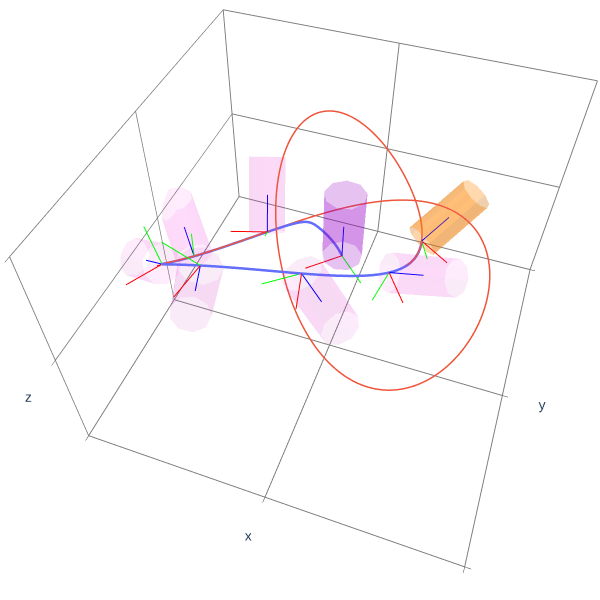
\includegraphics[width=0.32\textwidth]{../figures/adaptive_traj1.pdf}}\quad
        \subfloat{\label{bb}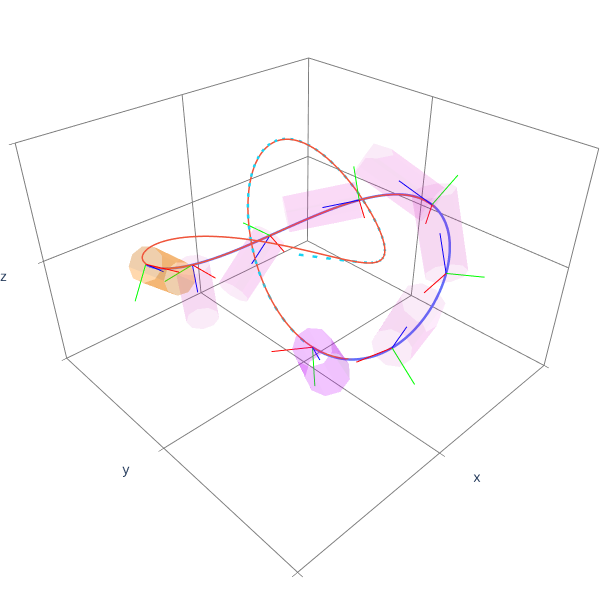
\includegraphics[width=0.32\textwidth]{../figures/adaptive_traj2.pdf}}
        \subfloat{\label{cc}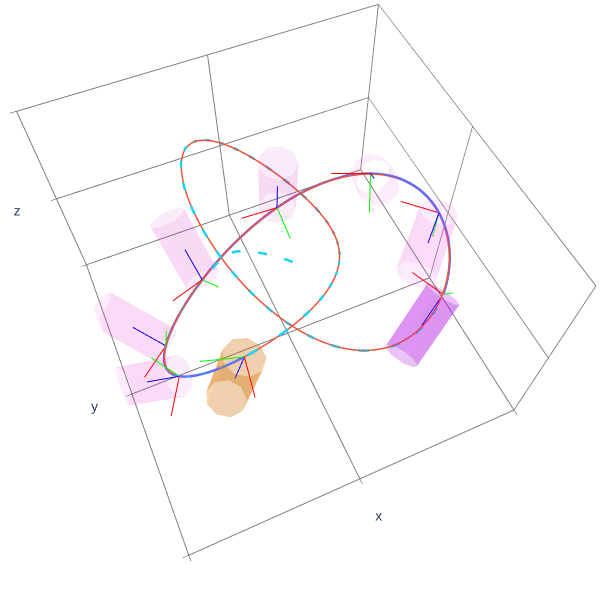
\includegraphics[width=0.32\textwidth]{../figures/adaptive_traj3.pdf}}
    \end{figure}
\end{frame}


\begin{frame}{Velocity error}
    \begin{figure}[ht!]
        \centering
        \def\svgwidth{.9\linewidth}
        {\scriptsize\import{../figures/}{adaptive_snorm.pdf_tex}}
    \end{figure}
\end{frame}

\begin{frame}{Distance}
    \begin{figure}[ht!]
        \centering
        \def\svgwidth{.9\linewidth}
        {\scriptsize\import{../figures/}{adaptive_distances.pdf_tex}}
    \end{figure}
\end{frame}